\section{Intro to GW theory with a view to higher genus (Patrick Lei)}%
\label{sec:Intro to GW theory with a view to higher genus (Patrick Lei)}


\subsection{Introduction to GW theory}%
\label{sub:Introduction to GW theory}

For the virtual fundamental class construction, see~\cite{BehrendFantechi1997}; for the axioms and quantum cohomology, see~\cite{KM1994}.

The goal of these lectures is to discuss Gromov-Witten theory in a way that is amenable to doing calculations in higher genus. Gromov-Witten theory concerns itself with integrals on the moduli space \(\Mbar_{g,n}(X, \beta)\), where \(X\) is a smooth projective algebraic variety and \(\beta \in H_2(X, \Z)\) is an effective curve class. There is a diagram
\begin{equation*}
\begin{tikzcd}
    \mc{C} \ar{r}{f} \ar[bend right=20]{d}[swap]{\pi} & X \\
    \Mbar_{g,n}(X, \beta) \ar[bend right=20]{u}[swap]{\sigma_i} \ar{ur}[swap]{\on{ev}_i}
\end{tikzcd}
\end{equation*}
where \(\mc{C}\) is the universal curve, \(\sigma_i\) are the sections of \(\pi\) which give the marked points, \(f\) is the universal stable map, and \(\ev_i = f \circ \sigma_i\) are evaluation morphisms. While \(\Mbar_{g,n}(X, \beta)\) is generally singular, not equidimensional, and reducible, there is a special class
\[ [\Mbar_{g,n}(X, \beta)]^{\vir} \in A_{\ab(c_1(X), \beta) + (\dim X - 3)(1-g) + n}(\Mbar_{g,n}(X, \beta), \Q), \]
which is known as the \textit{virtual fundamental class}. 

\begin{exer}
    Use standard arguments in deformation theory to verify that the ``expected dimension'' of \(\Mbar_{g,n}(X, \beta)\) is the number given above.
\end{exer}

Under the assumption that \(X\) is smooth and projective, \(\Mbar_{g,n}(X, \beta)\) is proper, so we may define \textit{GW invariants}
\[ \ab<\tau_{a_1}(\alpha_1), \cdots, \tau_{a_n}(\alpha_n)>_{g,n,\beta} \coloneqq \int_{[\Mbar_{g,n}(X, \beta)]^{\vir}} \prod_{i=1}^n \ev_i^* \alpha_i \cdot \psi_i^{a_i} \]
for \(\alpha_i \in H^*(X)\). Here, the \(\psi_i\) are defined by \(\psi_i = c_1(\sigma_i^*(\omega_{\pi}))\).

Unfortunately, calculating individual Gromov-Witten invariants is very difficult, so we will consider the even more difficult problem of studying generating series of GW invariants, for example
\[ F_g = \sum_{\beta \geq 0} q^{\beta} \ab<>_{g,0,\beta} \]
when \(X\) is a Calabi-Yau threefold. Here, \(q\) is a formal variable which keeps track of the curve class and we will denote the ring \(\Q\ps{q^{\beta} \mid \beta \in H_2(X, \Z)_{\mr{eff}}}\) by \(\Lambda\). There are some other structures we will consider. First, we may consider the \textit{quantum cohomology ring}, whose product \(a \star_{\mbf{t}} b\) is given by the formula 
\[
    (a \star_{\mbf{t}} b, c) = \sum_{\substack{\beta \geq 0 \\ n \geq 0}} \ab<a,b,c, \mbf{t}, \ldots, \mbf{t}>_{0,3+n,\beta} \frac{q^{\beta}}{n!}.
\]
Here \(a,b,c, \mbf{t} \in H^*(X)\). We will also consider the \textit{quantum connection}. Let \(\ab\{ e_i \}\) be a basis for \(H^*(X)\). Then the quantum connection is the connection on the trivial bundle with fiber \(H^*(X)\) over \(H^*(X) \times \P^1_z\) given by the formula
\[ \nabla_{t^i} = \partial_{t^i} + \frac{1}{z} e_i \star_{\mbf{t}}. \]
Sometimes, it is useful to also consider the connection in the \(z\)-direction given by 
\[ \nabla_{z \odv{}{z}} \coloneqq z \odv{}{z} - \frac{1}{z} E_X \star_{\mbf{t}} + \mu_X, \]
where \(\mu_X(\alpha) = \frac{\deg(\alpha) - \dim X}{2} \alpha\) is the grading operator and
\[ E_X = c_1(X) + \sum_i \ab(1 - \frac{\deg(e_i)}{2})t^i e_i \]
is the \textit{Euler vector field}. Because we will be mostly interested in Calabi-Yau varieties, we will not consider this.

\subsection{Enumerative mirror symmetry in genus zero}%
\label{sub:Enumerative mirror symmetry in genus zero}

The impetus for mathematicians to develop and study Gromov-Witten theory came in the early 1990s, when Candelas, de la Ossa, Green, and Parkes~\cite{CandelasEtAl1991} predicted the number of rational curves of low degree on a general quintic threefold by converting the problem to one of computing period integrals on a different Calabi-Yau threefold called the \textit{mirror quintic} (equivalently, studying its variation of Hodge structure). In genus zero, all invariants can be recovered from the \textit{J-function} \(J_{\mbf{t}}(q,z) \in H^*(X, \Lambda)[z]\), which is defined by
\[ \ab( J_{\mbf{t}}(q, z), \alpha ) \coloneqq (z + \mbf{t}, \alpha) + \sum_{n, \beta} \frac{q^{\beta}}{n!} \ab< \frac{\alpha}{z-\psi}, \mbf{t}, \ldots, \mbf{t}>_{0,1+n, \beta} \]
for any \(\mbf{t} \in H^*(X, \Lambda)[z]\) and \(\alpha \in H^*(X)\), where \((-,-)\) is the Poincar\'e pairing. Therefore, the problem of computing all genus-zero Gromov-Witten invariants with descendants (these are the \(\psi\)-classes) reduces to the problem of computing the J-function.

\begin{rmk}
    We expand \(\frac{1}{z-\psi}\) as \(\sum_{k=0}^{\infty} \psi^k z^{-k-1}\).  
\end{rmk}

We should note that the J-function can be obtained via a fundamental solution to the quantum differential equation, which is given by
\[ ( S_{\mbf{t}}(z) \phi , \alpha) = (\phi, \alpha) + \sum_{n, \beta} \frac{q^{\beta}}{n!} \ab<\frac{\alpha}{z-\psi}, \phi, \mbf{t}, \ldots, \mbf{t}>_{0, 2+n, \beta}. \]
This has the property that \(S_{\mbf{t}}^*(-z) S_{\mbf{t}}(z) = \on{Id}\), which is usually known as the \textit{symplectic property}. From this, we can recover the J-function by \(z S_{\mbf{t}}^*(z)\cdot 1 = J_{\mbf{t}}(q, z)\).

In physics, mirror symmetry is a duality between two different theories called the A-model and B-model, so now we will need to introduce the B-model object. In the interest of time (and notation), we will assume that \(X\) is a toric variety and that \(-K_X\) is nef. Let \(D_1, \ldots, D_r\) be the complete set of torus-invariant divisors in \(X\). Then define the \(I\)-function
\[
    I_{\mbf{t}}(q, z) \coloneqq z e^{\mbf{t}/z} \sum_{\beta \geq 0} q^{\beta} \frac{\prod_{i=1}^r \prod_{m = -\infty}^{0} (D_i + mz)}{\prod_{i=1}^r \prod_{m=-\infty}^{\beta \cdot D_i} (D_i + mz)}.
\]
Note here that we expand any \((D_i + mz)^{-1}\) which appears as \(\frac{1}{mz} \ab(1 - \frac{D_i}{mz} + \cdots)\), or namely, as a geometric series in \(\frac{D_i}{mz}\). In addition, the I-function is annihilated by a differential equation known as the \textit{Picard-Fuchs equation}, which is some hypergeometric type equation.

\begin{exm}
    If \(\mbf{t} = 0\) and \(X = \P^1\), we obtain
    \begin{align*}
        I(q,z) &= z\sum_{d \geq 0} q^d \frac{1}{\prod_{m=1}^d (H + mz)^2} \\
        &= z\sum_{d \geq 0} \ab(\frac{q}{z^2})^d \frac{1}{(d!^2)} + O(H),
    \end{align*}
    so in fact we see the Bessel function of the first kind as the leading term.
\end{exm}

If \(X\) is a complete intersection in a toric variety \(Y\) cut out by line bundles \(L_1, \ldots, L_k\), all of which satisfy \(H^1(f^* L_i) = 0\) for any genus zero stable map to \(Y\) (this is called being \textit{convex}), then the quantum Lefschetz theorem~\cite{CoatesGivental2007} allows us to replace \([\Mbar_{g,n}(X, \beta)]^{\vir}\) with \(e\ab(\bigoplus \pi_* f^* L_i) \cap [\Mbar_{g,n}(Y, \beta)]^{\vir}\) and perform all computations on \(Y\). In this case, the I-function is defined to be
\[
    I_{\mbf{t}}(q,z) \coloneqq z e^{\mbf{t}/z} \sum_{\beta \geq 0} q^{\beta} \frac{\prod_{i=1}^k \prod_{m=-\infty}^{L_i \cdot \beta} (L_i + mz)}{\prod_{i=1}^k \prod_{m=-\infty}^{0} (L_i + mz)} \frac{\prod_{i=1}^r \prod_{m = -\infty}^{0} (D_i + mz)}{\prod_{i=1}^r \prod_{m=-\infty}^{\beta \cdot D_i} (D_i + mz)},
\]
where we abuse notation and conflate the \(L_i\) with their first Chern classes.

\begin{exm}
    For the quintic threefold, which is cut out by a section of \(\mc{O}_{\P^4}(5)\), the I-function at \(\mbf{t} = 0\) is given by
    \[ I(q,z) = z \sum_{d \geq 0} q^d \frac{\prod_{m=1}^{5d}(5H+mz)}{\prod_{m=1}^d (H+mz)^5}. \]
\end{exm}

The content of the genus zero mirror theorem is a correspondence between these two objects. More precisely, in the case where \(-K_X\) is nef, they are related by a change of variables.

\begin{thm}[{\cite{Givental1998,LLY1997}}]
    Write the I-function with \(\mbf{t} = 0\) as \(I_0(q) \cdot z + I_1(q) + O(z^{-1})\). Then we have 
    \[
        J_{\tau(\mbf{t})}(q,z) = \frac{I_{\mbf{t}}(q,z)}{I_0(q)},
    \]
    where \(\tau(\mbf{t}) = \frac{\mbf{t} + I_1(q)}{I_0(q)}\). 
\end{thm}

\begin{exm}
    When \(X = \P^1\), note that \(I_0(q) = 1\) and \(I_1(q) = 0\), so in fact, we have the equality
    \[ J_{\mbf{t}}(q,z) = I_{\mbf{t}}(q,z). \]
\end{exm}

\begin{exm}
    When \(X\) is the quintic threefold, we will rewrite the components of the I-function as \(I_0(q) \cdot z + I_1(q)H + O(z^{-1})\) for convenience. We have
    \[ I_0(q) = \sum_{d \geq 0} \frac{(5d)!}{(d!)^5} q^d, \qquad I_1(q) = \sum_{d \geq 0} \frac{(5d)!}{(d!)^5} \ab(5\sum_{m=d+1}^{5d} \frac{1}{m}) q^d, \]
    so there is a nontrivial mirror map in this case. Specializing to \(\mbf{t} = 0\), we see that \(\tau = \frac{I_1(q)H}{I_0(q)}\), so we obtain
    \[ J_{\tau}(q,z) = \frac{I(q,z)}{I_0(q)}. \]
    By the divisor equation, the left hand side also equals \(J(qe^{I_1/I_0}, z)\), and we will also refer to this as the mirror map.  
    Therefore, we can use the mirror theorem to compute $\star_{\tau}$. The quantum connection in the direction of \(H^2\) becomes the ODE
    \[ (H+zD) S_{\tau}(z)^* = S_{\tau}(z)^* \cdot I_{11} H \star_{\tau}, \]
    where $D \coloneqq q \odv{}{q}$ (here, the coordinate is $\log q$) and $I_{11} \coloneqq 1 + D \ab(\frac{I_1(q)}{I_0(q)})$. An explicit computation using the mirror theorem and the results of Zagier--Zinger~\cite{ZagierZinger2008} yields
    \begin{align*}
        I_{11} H + \cdots &= S_{\tau}(z)^* (I_{11} H \star_{\tau} \1) \\
        \ab( 1 + D\ab(\frac{\frac{I_1}{I_0} + D \ab(\frac{I_2}{I_0})}{I_{11}}) ) H^2 + \cdots &= S_{\tau}(z)^* (I_{11} H \star_{\tau} H) \\
        I_{11} H^3 &= S_{\tau}(z)^* (I_{11}H \star_{\tau} H^2).
    \end{align*}
    Because $S_{\tau}$ begins with the identity, this computes $H \star_{\tau}$.
\end{exm}

\subsubsection{Oscillating integrals}%
\label{ssub:Oscillating integrals}

We will now reinterpret the genus zero mirror theorem, and we will return to this interpretation when we discuss higher genus invariants. In particular, we will interpret the I-function as an integral on some mirror family to \(X\), which for us will be a toric variety. Let
\[ 0 \to \Lambda \to \Z^r \to N \to 0 \]
be the fan sequence of \(X\). Applying \(\Hom(-, \C^{\times})\), we obtain the exact sequence
\[ 1 \to (\C^{\times})^{\dim X} \to (\C^{\times})^r \to \Hom(\Lambda, \C^{\times}) \to 1. \]
Suppose that the map \(\Lambda \to \Z^r\) is given by the matrix \((m_{ij})_{i=1,\ldots,r}^{j = 1, \ldots, \rho(X)}\). Then we consider the variety
\[ E_q = \ab(\prod_{i=1}^r x_j^{m_{ij}} = q_i \middle\vert i=1, \ldots, \rho(X)) \]
which is mirror to \(X\) and consider the superpotential \(f = x_1 + \cdots + x_r\). If we wish to consider the equivariant theory with equivariant parameters \(\lambda_1, \ldots, \lambda_r\) acting on each homogeneous coordinate of \(X\), we will consider \(f_{\lambda} = \sum_{i=1}^r (x_i - \lambda_i \log x_i)\). 

\begin{exm}
    When \(X = \P^n\), the mirror to \(X\) is the superpotential \(\sum_{i=1}^{n+1} (x_i - \lambda_i \log x_i)\) on the variety \(E_q = (x_1 \cdots x_{n+1} = q)\).   
\end{exm}

We now choose an appropriate Lefschetz thimble \(\Gamma_{\alpha}\) near each critical point \((x_{\alpha})\) of the (equivariant) superpotential and consider the integral
\[ I_{\alpha} = \int_{\Gamma_{\alpha}} e^{f_{\lambda}/z} \prod_{i=1}^r \frac{\d{x_i}}{x_i}. \]
This corresponds in the I-function to replacing each \(D_i\) in the expression by \(D_i - \lambda_i\) (turning on the equivariant parameters) and in the J-function to considering the fully equivariant GW theory of \(X\). In genus zero, the limit as \(\lambda_i \to 0\) exists, so we can safely recover the original mirror theorem from the following:

\begin{thm}[{\cite{Givental1996}}]
    This integral is annihilated by the same Picard-Fuchs equation as the I-function, and up to various prefactors, its asymptotic expansion as \(z \to 0^-\) along the negative real axis coincides with the restriction of the I-function corresponding to the T-fixed point on \(X\) which corresponds to the critical point \(( x_{\alpha} )\). 
\end{thm}


\subsubsection{The Lagrangian cone}%
\label{ssub:The Lagrangian cone}

The quantum cohomology of \(X\) is an example of a \textit{Frobenius manifold}, which we will see later can be produced from any cohomological field theory. Write \(V = H^*(X)\) and let \((e_{\mu})\) be a basis for \(V\), so we can write $\bv = \sum_{\mu,n} t^{\mu}_n e_{\mu} z^n \in V\ps{z}$.
The structure of a Frobenius manifold comes from the function
\[
    \mc{F}_0(\bv) = \sum_{n, \beta, \mu} \frac{q^{\beta}}{n!} \ab<\bv(\psi), \ldots, \bv(\psi)>_{0,n,\beta},
\]
which is also called the \textit{genus zero descendant potential} of \(X\). It satisfies the string equation, dilaton equation, and topological recursion relations: 
\begin{align*}
    \pdv{}{t_0^1} \mc{F}_0 &= \frac{1}{2} (\bv_0, \bv_0) + \sum_{n=0}^{\infty} \sum_{\mu} t_{n+1}^{\mu} \pdv{}{t_n^{\mu}} \mc{F}_0; \\
    \pdv{}{t_1^1} \mc{F}_0 &= \sum_{n=0}^{\infty} \sum_{\mu} t_n^{\mu} \pdv{}{t_n^{\mu}}\mc{F}_0 - 2 \mc{F}_0; \\
    \pdv{}{t_{k+1}^{\alpha},t_m^{\beta},t_n^{\gamma}} \mc{F}_0 &= \sum_{\mu,\nu} \pdv{}{t_k^{\alpha},t_0^{\mu}} \mc{F}_0 \cdot \eta^{\mu\nu} \cdot \pdv{}{t_0^{\nu},t_{m}^{\beta},t_n^{\gamma}} \mc{F}_0.
\end{align*}
To state the following result, we consider the infinite-dimensional vector space $V\ls{z^{-1}}$ (or a completion of this) with the symplectic form
\[ \omega(\mbf{f}(z), \mbf{g}(z)) \coloneqq \on{Res}_{z=0}(\mbf{f}(-z), \mbf{g}(z)). \]
We also consider the new variable\footnote{This is called the \textit{dilaton shift}.} $\bq = \bv - z$, so $\mc{F}_0$ is now a function near $\bq = -z$.

\begin{thm}[Givental {\cite{Givental2004}}]
    $\mc{F}_0$ satisfies the above PDEs if and only if the graph $\mc{L}$ of $\d{\mc{F}_0}$ is a Lagrangian cone with vertex at $\bq = 0$ such that its tangent spaces $L$ are tangent to $\mc{L}$ exactly along $zL \subset L$.
\end{thm}

We may recover the Lagrangian cone $\mc{L}$ by the following procedure. We find a fundamental solution 
\[ S = \mr{Id} + S_1 z^{-1} + S_2 z^{-2} + \cdots \]
to the quantum connection, which satisfies the equation
\[ z \pdv{}{t^{\mu}}S = e_{\mu} \star S. \]
Then, setting $J \coloneqq z S^*(z) \1$, we can then recover the Lagrangian cone by the following procedure:
\begin{itemize}
    \item The derivatives $\pdv{}{t^{\mu}} J$ form a basis of $L \cap V\ps{z^{-1}}$;
    \item This implies that $z \pdv{}{t^{\mu},t^{\nu}} J \in L \cap V \ps{z^{-1}}$. Writing these in terms of the first derivatives and using the fact that $J$ solves the quantum connection, we recover the Frobenius structure and hence the Lagrangian cone.
\end{itemize}

Using this, we can interpret the genus zero mirror theorem as:
\begin{thm}[{\cite{Givental1998}}]
    The I-function \(I_{\mbf{t}}(q,z)\) lies on the Lagrangian cone of \(X\).
\end{thm}




\subsection{Moduli of curves and CohFTs}%
\label{sub:Moduli of curves and CohFTs}

The notion of a cohomological field theory was introduced by Kontsevich--Manin~\cite{KM1994}.

We will denote by $\Mbar_{g,n}$ the moduli space of stable curves of genus $g$ with $n$ marked points. This is nonempty if and only if $2g-2+n > 0$, in which case it is a Deligne-Mumford stack of dimension $3g-3+n$. There is a combinatorial structure to the collection of $\Mbar_{g,n}$, which is given by a collection of morphisms.
\begin{itemize}
    \item There is the gluing morphism 
        \[q \colon \Mbar_{g,n+1} \times \Mbar_{h, m+1} \to \Mbar_{g+h,n+m}, \] 
        which takes two curves and glues them along the last marked point to form a node;
    \item There is the self-gluing morphism \[s \colon \Mbar_{g-1,n+2} \to \Mbar_{g,n},\] 
        which glues the last two marked points.
\end{itemize}
There is of course another interesting map, which is the forgetful map
\[ \pr \colon \Mbar_{g,n+1} \to \Mbar_{g,n} \]
given by deleting the last marked point and then stabilizing. We are now able to define our enumerative theories of interest, which include Gromov-Witten theory.

\begin{defn}
    Given a vector space $V$ with a nondegenerate symmetric bilinear form $\eta$ and a unit element $\1 \in V$, a \textit{Cohomological Field Theory (CohFT)} $\Omega$ on $V$ is a collection $\Omega_{g,n}$ of $S_n$-equivariant linear maps
    \[ \Omega_{g,n} \colon V^{\otimes n} \to H^*(\Mbar_{g,n}) \]
    which satisfy the basic identity
    \[ \Omega_{0,3}(\1, u,v) = \eta(u,v) \]
    and the following combinatorial identities (we will let $e_{\mu}$ be a basis of $V$ such that $e_1 = \1$ and $e^{\mu}$ be the dual basis):
    \begin{align*}
        q^* \Omega_{g+h,n+m}(\bv_1, \bv_2) &= \sum_{\mu} \Omega_{g,n+1}(\bv_1, e_{\mu}) \cdot \Omega_{h,m+1}(  \bv_2, e^{\mu} ); \\
        s^* \Omega_{g,n}(\bv) &= \sum_{\mu} \Omega_{g,n+2}(\bv, e_{\mu}, e^{\mu}).
    \end{align*}
    If in addition the identity
    \[ \pr^*\Omega_{g,n}(\bv) = \Omega_{g,n+1}(\bv,\1) \]
    is satisfied, then we say the CohFT has a \textit{flat unit} (or satisfies the \textit{string equation}).
\end{defn}
All of this can be generalized to super vector spaces, but for simplicity we will not deal with this case.

\begin{exm}
    The most important example of a CohFT is the Gromov-Witten theory of a smooth projective variety $X$. Here, recall that the source of a stable map is a \textbf{prestable} curve, so there is a stabilization morphism
    \[ \st \colon \Mbar_{g,n}(X,\beta) \to \Mbar_{g,n} \]
    which forgets the map and stabilizes the curve. Then, working over the Novikov ring, we will set $V = H^*(X)$, $\eta$ to be the Poincar\'e pairing, and $\1$ to be the fundamental class of $X$. The linear maps $\Omega^X_{g,n}$ are given by the formulae
    \[ \Omega_{g,n}^X(\btau) \coloneqq \sum_{\beta} q^{\beta} \st_* \ab(\prod_{i=1}^n \ev_i^*(\tau_i) \cap [\Mbar_{g,n}(X,\beta)]^{\vir}), \]
    where $\ev_i \colon \Mbar_{g,n}(X,\beta) \to X$ is the $i$-th evaluation map.
\end{exm}

\begin{exm}
    Let $\pi \colon \mc{C}_{g,n} \to \Mbar_{g,n}$ be the universal curve. Then the \textit{Hodge bundle} is the vector bundle 
    \[ \E_{g,n} \coloneqq \pi_* \omega_{\pi}. \]
    We then consider the vector space $V = \C$ with the usual pairing and define the CohFT $\Omega^{\E}$ by the formula
    \[ \Omega^{\E}_{g,n} \coloneqq c(\E_{g,n}). \]
    The gluing axioms are satisfied by the equation $q^* \E_{g+h} = \E_g \oplus \E_h$ and the exact sequence
    \[ 0 \to \E_{g-1} \to \E_g \to \mc{O} \to 0. \]
    Here, because genus zero components do not contribute to global sections of $\omega$ and $\E$ does not depend on the marked points, this CohFT has a flat unit.
\end{exm}

\begin{rmk}
    We will see later that this is related to the GW CohFT of a point by the quantum Riemann-Roch theorem. 
\end{rmk}

Given a CohFT $\Omega$, we may produce invariants by pairing the classes $\Omega_{g,n}(\bv)$ with various cohomology classes on $\Mbar_{g,n}$. The most important ones to consider are the classes
\[ \bar{\psi}_i \coloneqq c_1( s_i^* \omega_{\pi} ), \]
where $s_i \colon \Mbar_{g,n} \to \mc{C}_{g,n}$ is the $i$-th marked point.

\begin{rmk}
    In Gromov-Witten theory, these are called \textit{ancestors}. There are also descendants, which are given by the same formula except using the moduli space $\mf{M}_{g,n}$ of prestable curves instead of $\Mbar_{g,n}$, where we factor the morphism $\st$ defined above as
    \[ \Mbar_{g,n}(X,\beta) \xrightarrow{\text{forget map}} \mf{M}_{g,n} \xrightarrow{\text{stabilize}} \Mbar_{g,n}. \]
    The descendant classes are denoted by $\psi_i$.
\end{rmk}

\begin{exm}
    We will calculate an invariant which will appear in the GW theory of Calabi-Yau threefolds. For any CohFT $\Omega$, consider the invariant
    \[ \ab<\1\bar{\psi}_1>_{1,1}^{\Omega}\coloneqq \int_{\Mbar_{1,1}} \Omega_{1,1}(\1)\bar{\psi}_1. \]
    Using the second gluing equation, the degree zero part of $\Omega_{1,1}(\1)$ is equal to
    \[ \sum_{\mu} \Omega_{0,3}(\1, e_{\mu}, e^{\mu}) = \sum_{\mu} \eta(e_{\mu}, e^{\mu}), \]
    which yields the (graded) dimension $\chi(V)$ of $V$ (for example, if \(V = H^*(X)\) for a Calabi-Yau threefold \(X\), this is the topological Euler characteristic of \(X\)). Therefore, we obtain
    \[ \ab<\1\bar{\psi}_1>_{1,1}^{\Omega} = \frac{\dim V}{24}. \]
\end{exm}

\begin{exm}
    Consider the GW CohFT of a point. This is given by $V = \C$ with the usual pairing and the formula 
    \[ \Omega_{g,n} = 1. \]
    Then we define the invariants
    \[ \ab<\bar{\psi}_1^{a_1} \cdots \bar{\psi}_n^{a_n}>_{g,n} \coloneqq \int_{\Mbar_{g,n}} \Omega_{g,n} \cdot \bar{\psi}_1^{a_1} \cdots \bar{\psi}_n^{a_n}. \]
    \begin{thm}[Kontsevich {\cite{Kontsevich1992}}]
        The function
        \[ \mc{D} \coloneqq \exp \ab(\sum_{g,n} \frac{\hbar^{g-1}}{n!}\sum_{a_1 + \cdots + a_n = 3g-3+n} \ab<\bar{\psi}_1^{a_1} \cdots \bar{\psi}_n^{a_n}>_{g,n} t_{a_1}\cdots t_{a_n}) \]
        is annihilated by the operators
        \begin{align*}
            L_{-1} \coloneqq{}& -\pdv{}{t_0} + \frac{\hbar^{-1}}{2} t_0^2 + \sum_{i=0}^{\infty} t_{i+1} \pdv{}{t_i};\\
            L_0 \coloneqq{}& -\frac{3}{2} \pdv{}{t_1} + \sum_{i=0}^{\infty} \frac{2i+1}{2} t_i \pdv{}{t_i} + \frac{1}{16};\\
            L_n \coloneqq{}& -\frac{(2n+3)!!}{2^{n+1}} \pdv{}{t_{n+1}} + \sum_{i=0}^{\infty} \frac{(2i+2n+1)!!}{(2i-1)!! 2^{n+1}} t_i \pdv{}{t_{i+n}} \\
            &+ \frac{\hbar}{2} \sum_{i=0}^{n-1} \frac{(2i+1) (2i-1) \cdots (2i+1-2n)}{2^{n+1}} \pdv{}{t_i,t_{n-1-i}}.
        \end{align*}
    \end{thm}
\end{exm}

\begin{rmk}
    This result (Virasoro constraints for a point) is equivalent to $\mc{D}$ being a tau-function for the KdV hierarchy and has been generalized by various authors.
\end{rmk}



\subsection{$R$-matrix action}%
\label{sub:R-matrix action}

In the early 2000s, Givental discovered a remarkable property of axiomatic enumerative theories, namely that one can transform CohFTs by the action of matrices $R(z) = R_0 + R_1 z + R_2 z^2 + \cdots \in \Hom(V, V')\ps{z}$ which satisfy the property
\[ R^*(-z) R(z) = \mr{Id}_V. \]
Traditionally, the literature requires that $V = V'$ and $R_0 = \mr{Id}$, but the MSP group has removed this restriction and also allows $\dim V < \dim V'$.

In order to define the action of $R$ on a CohFT $\Omega$ defined on $V$, we need to review some of the combinatorial structure of $\Mbar_{g,n}$. For a curve $C\in \Mbar_{g,n}(\C)$, we may consider the dual graph of $C$, which has vertices, edges, and legs, which are defined as follows:
\begin{itemize}
    \item The vertices correspond to irreducible components of $C$ and are labelled by a non-negative integer, which is the genus;
    \item The edges correspond to nodes of $C$ (in particular, we allow loops);
    \item The legs correspond to marked points.
\end{itemize}
Any graph which appears as the dual graph of a stable curve is called a \textit{stable graph}.

\begin{figure}[htpb]
  \centering
  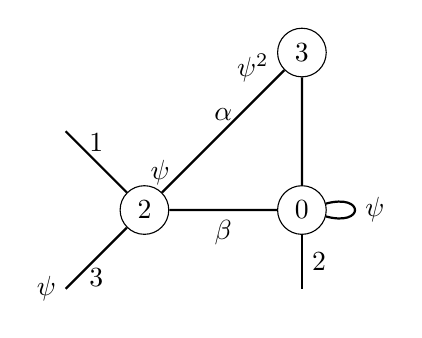
\begin{tikzpicture}[scale=1,transform shape,every loop/.style={}]
    \node[circle,draw] (A) at (0,0) {$2$};
    \node[circle,draw] (B) at (2,2) {$3$};
    \node[circle,draw] (C) at (2,0) {$0$};
    \draw[thick] (A) -- node[above]{$\alpha$} (B) -- (C) -- node[below]{$\beta$} (A);
    \draw[thick] (A) -- node[below]{$3$} (-1,-1);
    \draw[thick] (A) -- node[above]{$1$} (-1,1);
    \draw[thick] (C) -- node[right]{$2$} (2,-1);
    \draw[thick] (C) edge[loop right] node[right] {$\psi$} (C);
    \node[anchor=east] at (-1,-1) {$\psi$};
    \node[anchor=east] at (1.7,1.8) {$\psi^2$};
    \node[anchor=south] at (0.2,0.2) {$\psi$};
  \end{tikzpicture}
  \caption{Example of a stable graph in $\ol{\mc{M}}_{7,3}$ and associated tautological class. This stable graph describes the image of a map
    $\ol{\mc{M}}_{2,4} \times \ol{\mc{M}}_{3,2} \times \ol{\mc{M}}_{0,5} \to \ol{\mc{M}}_{7,3}$.}
  \label{fig:stablegraph}
\end{figure}

The first type of action on CohFTs is a translation action. Let $T \in V\ps{z}$. For a CohFT $\Omega$, we define
\[ (T\Omega)_{g,n}(\bv) \coloneqq \sum_m \frac{1}{m!} p_* \Omega_{g,n+m}(\bv, T,\ldots,T) \]
whenever the infinite sum makes sense.

\begin{exm}
    If $\Omega^X$ is the GW CohFT of a smooth projective variety $X$ and $\tau \in H^2(X)$ is a divisor class, then the infinite sum makes sense and we can define the shifted GW CohFT $\Omega^{X,\tau}$ of $X$. For example, if $X$ is the quintic threefold and $\tau = \frac{I_1}{I_0} H$, then shifting to $\tau$ is the same as the mirror map $q \mapsto Q(q) = q e^{\frac{I_1}{I_0}}$.
\end{exm}

The second type of action is the action of a matrix $R$ as in the beginning of this section. Let $G_{g,n}$ denote the set of all stable graphs of genus $g$ with $n$ legs. Then we define
\[ (R\Omega)_{g,n} \coloneqq \sum_{\Gamma \in G_{g,n}} \frac{1}{\ab|\Aut \Gamma|} \on{Cont}_{\Gamma}, \]
where $\on{Cont}_{\Gamma}$ is defined by the following construction:
\begin{itemize}
    \item At the $i$-th leg, we place the map 
        \[ R(-\bar{\psi}_i)^* \in \Hom(V',V) \ps{\bar{\psi}_i}; \]
    \item At every edge, we place the bivector
        \[ V(\bar{\psi}_1, \bar{\psi}_2) \coloneqq \sum_{\mu} \frac{e_{\mu} \otimes e^{\mu} - R(-\bar{\psi}_1)^* e_{\mu} \otimes R(-\bar{\psi}_2)^* e^{\mu}}{\bar{\psi}_1 + \bar{\psi}_2}; \]
    \item At every vertex, we place the linear map
        \[ \Omega_{g_v, n_v} \colon V^{\otimes n_v} \to H^*(\Mbar_{g_v, n_v}); \]
    \item Finally, we consider the pushforward in cohomology along the gluing morphism $\prod_v \Mbar_{g_v, n_v} \to \Mbar_{g,n}$.
\end{itemize}

\begin{defn}
    Let $R$ be as above. Then we define the translation
    \[ T_R \coloneqq z (\1 - R(-z)^* \1') \in z V\ps{z}. \]
    Whenever it makes sense, we define
    \[ R.\Omega \coloneqq RT\Omega. \]
\end{defn}

\begin{thm}[Chang-Guo-Li {\cite[Theorem~2.7]{CGL2026}}]
    Suppose we work with coefficients in $\C\ps{q}$. Then if
    \[ T_R \in z^2 V \ps{z} + zq V \ps{z}, \]
    $R.\Omega$ is a well-defined CohFT. Moreover, if $\dim V = \dim V'$, $\1'$ is a unit for $R.\Omega$.
\end{thm}

We would like to remark a bit more about the translation action when $R_0 \neq \mr{Id}$. For simplicity, we will assume that $V = V'$ and $R_0 \1 = c \cdot \1$ for some constant $c$. Then we set $\tilde{T}_R \coloneqq z( \1 - c R(z)^{-1} \1)$ and use the dilaton equation to compute
\begin{align*}
    T_R \Omega_{g,n}(\bv) &= \sum_{m=0}^{\infty} \frac{1}{m!} p_*\Omega_{g,n+m}(\bv, T_R, \ldots, T_R) \\
    &= \sum_{k,\ell \geq 0} \frac{1}{k!\ell!} p_* \Omega_{g,n+k+\ell}(\bv, ( (1-c^{-1})\1 \cdot \psi )^{\otimes k}, ( c^{-1} \tilde{T}_R )^{\otimes \ell}) \\
    &= \sum_{k,\ell \geq 0} \frac{(1-c^{-1})^k \cdot c^{-\ell}}{\ell!} \binom{2g-2+n+k+\ell-1}{k} p_* \Omega_{g,n+\ell}(\bv, \tilde{T}_R^{\otimes \ell}) \\
    &= \sum_{m=0}^{\infty} \frac{c^{2g-2+n}}{m!} p_* \Omega_{g,n+m}(\bv, \tilde{T}_R, \ldots, \tilde{T}_R)
\end{align*}
whenever this makes sense.


